\section{Relating synchronisation linearisation and linearisation}
\label{sec:relating}

In this section we describe the relationship between synchronisation
linearisation and standard linearisation.  

It is clear that standard linearisation is equivalent to synchronisation
linearisation in the (rather trivial) case that no operations synchronise, so
each operation of the synchronisation specification object corresponds to a
single operation of the concurrent object.  Put another way: standard
linearisation is an instance of synchronisation linearisation. 

%% Below, we show that the two notions
%% are different: synchronisation linearisation cannot, in general, be captured
%% directly as standard linearisation.  However, we show that synchronisation
%% linearisation corresponds to a small adaptation of linearisation, where one of
%% the operations of the synchronisation object corresponds to \emph{two}
%% operations of the linearisation specification object.

However, linearisability and synchronisation linearisability are not
equivalent in general: we show that, given a synchronisation linearisability
specification object |SyncSpec|, it is not always possible to find a
linearisability specification |Spec| such that for every history~$h$,\, $h$ is
synchronisation linearisable with respect to |SyncSpec| if and only if $h$ is
linearisable with respect to |Spec|.

For example, consider the example of a synchronous channel from
Section~\ref{sec:spec}, where synchronisation linearisation is captured by
|SyncChanSpec|.  Assume (for a contradiction) that the same property can be
captured by linerisation with respect to linearisability specification~|Spec|.
Consider the history
\begin{eqnarray*}
h & = & \seq{ 
  \call.\send^1(3), \call.\receive^2(), 
  \return.\send^1\::(), \return.\receive^2()\::3 }.
\end{eqnarray*}
%
This is synchronisation linearisable with respect to |SyncChanSpec|.  By the
assumption, it must also be linearisable with respect to~|Spec|; so there must
be a legal history~$h_s$ of~|Spec| such that $h$ and~$h_s$ are compatible.
Without loss of generality, suppose the |send| in~$h_s$ occurs before
the~|receive|, i.e.
\begin{eqnarray*}
h_s & = & \seq{ \send^1(3)\::(), \receive^2()\::3 }.
\end{eqnarray*}
%
But the history
%
\begin{eqnarray*}
h' & = & \seq{ 
  \call.\send^1(3), \return.\send^1\::(), 
  \call.\receive^2(), \return.\receive^2()\::3 }
\end{eqnarray*}
%
is also compatible with~$h_s$, so $h'$ is linearisable with respect to~|Spec|.
But then the assumption would imply that $h'$ is synchronisation linearisable
with respect to~|SyncChanSpec|.  This is clearly false, because the operations
do not overlap.  Hence no such linearisability specification~|Spec| exists.


%%%%%%%%%%%%%%%%%%%%%%%%%%%%%%%%%%%%%%%%%%%%%%%%%%%%%%%

\subsection{Two-step linearisability}

%% \framebox{Note: I don't think we want both this and the construction in
%%   Section~\ref{ssec:testing-hacking}.}

We now show that binary synchronisation linearisability corresponds to a small
adaptation of linearisability, where one of the operations on the concurrent
object corresponds to \emph{two} operations of the linearisability
specification object.  We define what we mean by this, and then prove the
correspondence in the next subsection; we generalise to synchronisations of
more than two threads in Section~\ref{ssec:relating-variations}.  In the
definitions below, we describe just the differences from standard
linearisation, to avoid repetition.

Given a synchronisation object with operations |op|\s1 and |op|\s2,
we will consider a linearisability specification object with signature
%
\begin{scala}
class TwoStepLinSpec{
  def op£\s1£(x£\s1£: A£\s1£): Unit
  def £$\overline{\sm{op}}_1$£(): B£\s1£
  def op£\s2£(x£\s2£: A£\s2£): B£\s2£
}
\end{scala}
%
The idea is that the operation |op|\s1 on the concurrent object will be
linearised by the composition of the two operations |op|\s1 and
$\overline{\sm{op}}_1$; but operation |op|\s2 on the concurrent object will be
linearised by just the operation |op|\s2 of the specification object, as
before.  We call such an object a \emph{two-step linearisability specification
  object}. 

We define a legal history~$h_s$ of such a two-step specification object much
as in Section~\ref{sec:specification-linearisability}, with the addition that
for each event $\overline{\sm{op}}_1^i()\::y$ in~$h_s$, we require that there
is an earlier event |op|$_1^i(x)\::()$ in~$h_s$ with the same invocation
identity; other than in this regard, invocation identities are not repeated
in~$h_s$.

Let $h$ be a complete concurrent history of a synchronisation object, and let
$h_s$ be a legal history of a two-step specification object corresponding to
the same invocations in the following sense:
%
\begin{itemize}
\item For every $\call.\sm{op}_1^i(x)$ and $\return.\sm{op}_1^i\::y$ in $h$,\,
  $h_s$~contains $\sm{op}_1^i(x)\::()$ and $\overline{\sm{op}}_1^i()\::y$; and
  vice versa;

\item For every $\call.\sm{op}_2^i(x)$ and $\return.\sm{op}_2^i\::y$ in $h$,\,
  $h_s$~contains $\sm{op}_2^i(x)\::y$; and vice versa.
\end{itemize}
%
We say that $h$ and $h_s$ are \emph{two-step-compatible} if there is some way of
interleaving the two histories such that 
%
\begin{itemize}
\item Each $\sm{op}_1^i(x)\::()$ and $\overline{\sm{op}}_1^i()\::y$ occur
  between $\call.\sm{op}_1^i(x)$ and $\return.\sm{op}_1^i\::y$, in that
  order; 

\item Each $\sm{op}_2^i(x)\::y$ occurs between $\call.\sm{op}_2^i(x)$ and
  $\return.\sm{op}_2^i\::y$.
\end{itemize}

For example, consider a synchronous channel, with |send| corresponding
to~$\op_1$, and |receive| corresponding to~$\op_2$.  Then the following would be
an interleaving of two-step-compatible histories of the synchronisation object
and the corresponding specification object.
\[
\seq{\begin{align} 
 \call.\sm{send}^1(3),\; \sm{send}^1(3)\::(),\; 
 \call.\sm{receive}^2(),\; \sm{receive}^2()\::3,\; \\
 \overline{\sm{send}}^1()\::(),\; \return.\sm{send}^1\::(), \;
 \return.\sm{receive}^2\::3 }.
\end{align}
\]
%
%\framebox{timeline to illustrate}
This is represented by the following timeline, where the horizontal lines and
the labels above represent the interval between the $\call$ and $\return$
events of the synchronisation object, and the ``$\cross$''s and the labels
below represent the corresponding operations of the specification object.
%  
\begin{center}
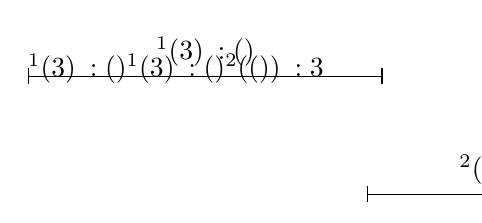
\begin{tikzpicture}[xscale = 0.9]
\draw[|-|] (0,0) -- node[above] {$\send^1(3)\::()$} (5,0);
\crossAt(1,0){$\send^1(3)\::()$}
\crossAt(4,0){$\overline{\send}^1(3)\::()$}
%\draw (1, 0) \X; \draw(4,0) \X;
\draw[|-|] (2,-1.5) -- node[above] {$\receive^2(())\::3$} (6,-1.5);
\crossAt(3,-1.5){$\receive^2(())\::3$}
%\draw(3,-1.5) \X;
\end{tikzpicture}
\end{center}

The definition of two-step linearisability then follows from this definition
of two-step compatability, precisely as in
Section~\ref{sec:specification-linearisability}.


%%%%%%%%%%%%%%%%%%%%%%%%%%%%%%%%%%%%%%%%%%%%%%%%%%%%%%%

\subsection{Proving the relationship}
\label{sec:twoStepLinSpec}

We now prove the relationship between synchronisation linearisation and
two-step linearisation.

Consider a synchonisation specification object |SyncSpec|.  We build a
corresponding two-step linearisation specification object~|TwoStepLinSpec|
such that synchronisation linearisation with respect to |SyncSpec| is
equivalent to two-step linearisation with respect to~|TwoStepLinSpec|.  The
definition we choose is not the simplest possible, but it is convenient for
the testing framework we use in Section~\ref{sec:testing-hacking}.  

The definition of |TwoStepLinSpec| is below.  We assume that each thread has
an identity in some range $\range 0 {\sm{NumThreads}}$.  For simplicity, we
arrange for this identity to be included in the $\call$ events written to the
log for operations~|op|\s1 and $\overline{\sm{op}}_1$.  (Alternatively, we
could implement thread identities internally to the object, for example using
the technique from~\cite[Appendix~A.2.4]{herlihy-shavit}.)

This object requires that corresponding invocations of~|op|\s1 and~|op|\s2 are
linearised consecutively: it does this by encoding the automaton on the right.
However, it allows the corresponding $\overline{\sm{op}}_1$ to be linearised
later (but before the next operation invocation by the same thread).  It uses
an array |returns|, indexed by thread identities, to record the value that
should be returned by an $\overline{\sm{op}}_1$ invocation by each thread.
Each invocation of $\op_2$ calls |SyncSpec.sync| to obtain the values that
should be returned for synchronisation linearisation; it writes the value for
the corresponding $\overline\op_1$ into |returns|.
%
\begin{trivlist}
\item[]
\begin{minipage}{92mm}
\begin{scala}
type ThreadID = Int               // Thread identifiers
val NumThreads: ThreadID = ... // Number of threads
trait State
case class Zero extends State
case class One(t: ThreadID, x£\s1£: A£\s1£) extends State
\end{scala}
\end{minipage}
%%%%%
\hfill 
%
\begin{minipage}{37.8mm}
\begin{tikzpicture}[>= angle 60, xscale = 0.9, yscale = 0.44]
\draw (0,0) node[draw] (zero) {$\sm{Zero}$};
\draw[->] (zero) ++ (-1.5, 0) -- (zero);
%
\draw (0,-4) node[draw] (one) {$\sm{One}(\sm t, \sm{x}_1)$};
\draw[->] (zero) .. controls ++(0.3,-2) .. 
  node[right] {$\sm{op}_1(\sm t, \sm{x}_1)$} (one); 
%
\draw[->] (one) .. controls ++(-0.3,2) .. 
  node[left] {$\sm{op}_2(\sm x_2)$} (zero);
\end{tikzpicture}%
\end{minipage}%
%%%%%
\begin{scala}
object TwoStepLinSpec{
  private var state: State = Zero
  private val returns = new Array[Option[B£\s1£]](NumThreads)
  for(t <- 0 until NumThreads) returns(t) = None
  def op£\s1£(t: ThreadID, x£\s1£: A£\s1£): Unit = {
    require(state.isInstanceOf[Zero] && returns(t) == None); state = One(t, x£\s1£); ()
  }
  def op£\s2£(x£\s2£: A£\s2£): B£\s2£ = {
    require(state.isInstanceOf[One]); val One(t, x£\s1£) = state
    val (y£\s1£, y£\s2£) = SyncSpec.sync(x£\s1£, x£\s2£); returns(t) = Some(y£\s1£); state = Zero; y£\s2£
  }
  def £$\overline{\sm{op}}_1$£(t: ThreadID): B£\s1£ = {
    require(state.isInstanceOf[Zero] && returns(t).isInstanceOf[Some])
    val Some(y£\s1£) = returns(t); returns(t) = None; y£\s1£
  }
}
\end{scala}
\end{trivlist}

%%%%%

%% \framebox{Do we want to talk about \emph{complete} histories of
%%   TwoStepDelayedLinSpec?} -- containing all three events of a set

The following lemma identifies important properties of
|Two|\-|Step|\-|Delayed|\-|LinSpec|.  It follows immediately from the
definition.
%
\begin{lemma}
\label{lem:TwoStepLinSpec-histories}
Within any legal history of |TwoStepDelayedLinSpec|, events $\op_1$ and
$\op_2$ alternate.  Let $\op_1^{i_1}(t,x_1) \:: ()$ and $\op_2^{i_2}(x_2) \::
y_2$ be a consecutive pair of such events.  Then |op|\s2 makes a call
$\sm{SyncSpec.sync}(x_1, x_2)$ obtaining result $(y_1,y_2)$.  The next event
for thread~$t$ (if any) will be $\overline\op_1^{i_1}(t) \:: y_1$; and this
will be later in the history than $\op_2^{i_2}(x_2) \:: y_2$.  Further, the
corresponding history of events $\sm{sync}^{i_1,i_2}(x_1,x_2) \:: (y_1,y_2)$
is a legal history of |SyncSpec|.

Conversely, each history with events ordered in this way will be a legal
history of |TwoStepDelayedLinSpec| if  the corresponding history
of events $\sm{sync}^{i_1,i_2}(x_1,x_2) \:: (y_1,y_2)$ is a legal history of
|SyncSpec|.
\end{lemma}

%%%%%

The following proposition reduces synchronisation linearisability to two-step
linearisability.
%
\begin{prop}
Let |SyncObj| be a synchronisation object, |SyncSpec| be a synchronisation
specification object, and let |TwoStepLinSpec| be built from |SyncSpec| as
above.  Then |SyncObj| is two-step linearisable with respect to
|Two|\-|Step|\-|LinSpec| if and only if it is synchronisation linearisable
with respect to |SyncSpec|.
\end{prop}
%%%%%%
\begin{proof}
\textbf{($\implies$).}\quad
%
Let $h$ be a concurrent history of |SyncObj|.  By assumption, there is an
extension $h'$ of~$h$, and a legal history~$h_s$ of |TwoStepLinSpec| such that
$h'' = complete(h')$ and~$h_s$ are two-step-compatible.
%
Build a history~$h_s'$ of |SyncSpec| by replacing each consecutive pair
$\sm{op}_1^{i_1}(x_1) \:: ()$,\, $\sm{op}_2^{i_2}(x_2) \:: y_2$ in~$h_s$ by
the event $\sm{sync}^{i_1,i_2}(x_1,x_2) \:: (y_1,y_2)$, where $y_1$ is the
value returned by the corresponding~$\overline{\sm{op}}_1^{i_1}()$.
%
This is illustrated by the example timeline below, where $h''$ is represented
by the horizontal lines and the labels above; $h_s$ is represented by the
``$\cross$''s and the labels below; and $h_s'$ is represented by the
``$\bullet$'' and the label below.
%
\begin{center}
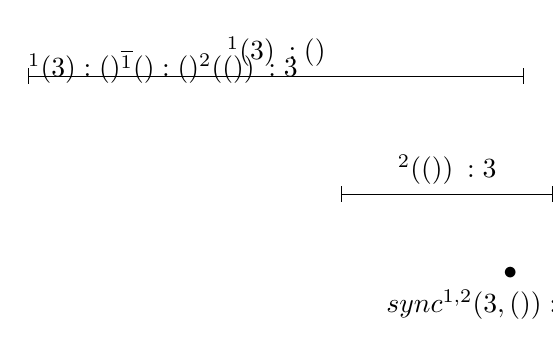
\begin{tikzpicture}[xscale = 0.9]
\draw[|-|] (0,0) -- node[above] {$\send^1(3)\::()$} (7,0);
\crossAt(1,0){$\send^1(3):()$}
%\draw (1, 0) \X; \draw (1,-0.4) node{$\sm{send}^1(3):()$}; 
\crossAt(6,0){$\overline{\send^1}():()$}
%\draw(6,0) \X; \draw(6,-0.4) node{$\overline{\sm{send}^1}():()$};
%
\draw[|-|] (2,-1.5) -- node[above] {$\receive^2(())\::3$} (5,-1.5);
\crossAt(3,-1.5){$\receive^2(())\::3$};
%\draw(3,-1.5) \X; \draw(3,-1.9) node{$\sm{receive}^2(())\::3$};
%
\draw(3,-2.5) node{$\bullet$}; 
\draw(3,-2.9) node{$\sm{sync}^{1,2}(3,()): ((),3)$};
\end{tikzpicture}
\end{center}

The history~$h_s'$ is legal for |SyncSpec| by
Lemma~\ref{lem:TwoStepLinSpec-histories}.
%
It is possible to interleave $h''$ and~$h_s'$ by placing each event
$\sm{sync}^{i_1,i_2}(x_1,x_2) \:: (y_1,y_2)$ in the same place as the
corresponding event $\sm{op}_2^{i_2}(x_2) \:: y_2$ in the interleaving
of~$h''$ and~$h_s$; by construction, this is between
$\call.\sm{op}_1^{i_1}(x_1)$ and~$\return.\sm{op}_1^{i_1} \:: y_1$, and
between $\call.\sm{op}_2^{i_2}(x_2)$ and~$\return.\sm{op}_2^{i_2} \:: y_2$.
%
Hence $h''$ and~$h_s$ are synchronisation-compatible; so $h''$ is
synchronisation-linearisable; and so $h$ is synchronisation-linearisable.

%%%%%

\textbf{($\Leftarrow$).}\quad
%
Let $h$ be a complete history of |SyncObj|.  By assumption, there is an
extension $h'$ of~$h$, and a legal history~$h_s$ of |SyncSpec| such that $h''
= complete(h')$ and~$h_s$ are synchronisation compatible.
%
Build a history~$h_s'$ of |TwoStepLinSpec| by replacing each event
$\sm{sync}^{i_1,i_2}(x_1,x_2) \:: (y_1,y_2)$ in~$h_s$ by the three consecutive
events $\sm{op}_1^{i_1}(x_1) \:: ()$,\, $\sm{op}_2^{i_2}(x_2) \:: y_2$,\,
$\overline{\sm{op}}_1^{i_1}() \:: y_1$.

The history~$h_s'$ is legal for |TwoStepLinSpec| by
Lemma~\ref{lem:TwoStepLinSpec-histories}.
%
It is possible to interleave $h''$ and~$h_s'$ by placing each triple
$\sm{op}_1^{i_1}(x_1) \:: ()$,\, $\sm{op}_2^{i_2}(x_2) \:: y_2$,\,
$\overline{\sm{op}}_1^{i_1}() \:: y_1$ in the same place as the corresponding
event $\sm{sync}^{i_1,i_2}(x_1,x_2) \:: (y_1,y_2)$ in the interleaving
of~$h''$ and~$h_s$; by construction, each $\sm{op}_1^{i_1}(x_1) \:: ()$ and
$\overline{\sm{op}}_1^{i_1}() \:: y_1$ are between
$\call.\sm{op}_1^{i_1}(x_1)$ and~$\return.\sm{op}_1^{i_1} \:: y_1$; and each
$\sm{op}_2^{i_2}(x_2) \:: y_2$ is between $\call.\sm{op}_2^{i_2}(x_2)$
and~$\return.\sm{op}_2^{i_2} \:: y_2$.
%
Hence $h''$ and~$h_s$ are two-step-compatible; so $h''$ is
two-step-linearisable; and so $h$ is two-step-linearisable.
\end{proof}

The two-step linearisation specification object can often be significantly
simplified from the template definition above.  Here is such a specification
object for a synchronous channel.
%
\begin{scala}
object SyncChanTwoStepLinSpec{
  private var state = 0           // Takes values 0, 1, cyclically 
  private var threadID = -1    // Current thread ID when state = 1
  private val canReturn =       // which senders can return?
    new Array[Boolean](NumThreads) 
  private var value: A = _      // The current value being sent
  def send(t: ThreadID, x: A): Unit = { 
    require(state == 0 && !canReturn(t)); value = x; threadID = t; state = 1 }
  def receive(u: Unit): A = { 
    require(state == 1); canReturn(threadID) = true; state = 0; value }
  def £$\overline{\send}$£(t: ThreadID): Unit = { 
    require(state == 0 && canReturn(t)); canReturn(t) = false }
}
\end{scala}

%%%%%%%%%%%%%%%%%%%%%%%%%%%%%%%%%%%%%%%%%%%%%%%%%%%%%%%

%% \subsection{Old version}

%% We now prove the relationship between synchronisation linearisation and
%% two-step linearisation.

%% Consider a synchonisation specification object |SyncSpec|.  We build a
%% corresponding two-step linearisation specification object~|TwoStepLinSpec|
%% such that synchronisation linearisation with respect to |SyncSpec| is
%% equivalent to two-step linearisation with respect to~|TwoStepLinSpec|.  The
%% definition is below: the specification's behaviour is described by the
%% automaton on the right.\footnote{Defining the subclasses of {\scalashape
%%     State} as {\scalashape case class}es allows pattern matching against such
%%   values.  For example, the statement {\scalashape val One(x}\s1{\scalashape )
%%     = state} succeeds only if {\scalashape state} has type {\scalashape One},
%%   and binds the name {\scalashape x}\s1 to the value of the {\scalashape x}\s1
%%   field of {\scalashape state}.}
%% \begin{trivlist}
%% \item[]
%% \begin{minipage}[b]{68mm}
%% \begin{scala}
%% trait State
%% case class Zero extends State
%% case class One(x£\s1£: A£\s1£) extends State
%% case class Two(y£\s1£: B£\s1£) extends State
%% \end{scala}
%% \end{minipage}
%% %
%% \hfil
%% %
%% \begin{minipage}[b]{63mm}
%% \begin{tikzpicture}[>= angle 60, xscale = 0.95, yscale = 0.75]
%% \draw (0,0) node[draw] (zero) {$\sm{Zero}$};
%% \draw[->] (zero) ++ (-1.5, 0) -- (zero);
%% %
%% \draw (4,0) node[draw] (one) {$\sm{One}(\sm{x}_1)$};
%% \draw[->] (zero)  -- node[above] {$\sm{op}_1(\sm{x}_1)$} (one); 
%% %
%% \draw (2, -2) node[draw] (two) {$\sm{Two}(\sm{y}_1)$};
%% \draw[->] (one)  -- node[right] {$\sm{op}_2(\sm{x}_2)$} (two); 
%% \draw[->] (two) -- node[left] {$\overline{\sm{op}}_1()$} (zero);
%% \end{tikzpicture}
%% \end{minipage}
%% %
%% %The specification object is defined as follows.
%% %
%% %% trait LinState
%% %% case class Zero extends LinState
%% %% case class One(x£\s1£: A£\s1£) extends LinState
%% %% case class Two(y£\s1£: B£\s1£) extends LinState
%% %
%% \begin{scala}
%% class TwoStepLinSpec{
%%   private var state: State = Zero
%%   def op£\s1£(x£\s1£: A£\s1£): Unit = {
%%     require(state.isInstanceOf[Zero]); state = One(x£\s1£)
%%   }
%%   def op£\s2£(x£\s2£: A£\s2£): B£\s2£ = {
%%     require(state.isInstanceOf[One]); val One(x£\s1£) = state
%%     val (y£\s1£, y£\s2£) = SyncSpec.sync(x£\s1£, x£\s2£); state = Two(y£\s1£); y£\s2£
%%   }
%%   def £$\overline{\sm{op}}_1$£(): B£\s1£ = {
%%     require(state.isInstanceOf[Two]); val Two(y£\s1£) = state; state = Zero; y£\s1£
%%   }
%% }
%% \end{scala}
%% \end{trivlist}
%% %
%% %
%% The definition forces the operations to take place in the order described by
%% the automaton.  In addition, the |op|\s2 operation calls the |sync| method on
%% |SyncSpec|, to calculate the return values and to update |SyncSpec|'s state;
%% it stores |op|\s1's result in the state. 

%% % in effect, the synchronisation happens at this point.

%% The following lemma follows immediately from the construction
%% of~|Two|\-|Step|\-|LinSpec|. 
%% %
%% \begin{lemma}
%% \label{lem:TwoStepLinSpec-historiesX}
%% Each history of~|TwoStepLinSpec| is the concatenation of triples of events of
%% the form $\sm{op}_1^{i_1}(x_1) \:: ()$,\, $\sm{op}_2^{i_2}(x_2) \:: y_2$,\,
%% $\overline{\sm{op}}_1^{i_1}() \:: y_1$  such that |SyncSpec| has a
%% corresponding legal history of events $\sm{sync}^{i_1,i_2}(x_1,x_2) \::
%% (y_1,y_2)$, and vice versa.
%% \end{lemma}

%% %%%%%

%% The following proposition reduces synchronisation linearisability to two-step
%% linearisability.
%% %
%% \begin{prop}
%% Let |SyncObj| be a synchronisation object, |SyncSpec| be a synchronisation
%% specification object, and let |TwoStepLinSpec| be built from |SyncSpec| as
%% above.  Then |SyncObj| is two-step linearisable with respect to
%% |Two|\-|Step|\-|LinSpec| if and only if it is synchronisation linearisable
%% with respect to |SyncSpec|.
%% \end{prop}
%% %%%%%%
%% \begin{proof}
%% \textbf{($\implies$).}\quad
%% %
%% Let $h$ be a concurrent history of |SyncObj|.  By assumption, there is an
%% extension $h'$ of~$h$, and a legal history~$h_s$ of |TwoStepLinSpec| such that
%% $h'' = complete(h')$ and~$h_s$ are two-step compatible.
%% %
%% Build a history~$h_s'$ of |SyncSpec| by replacing each triple
%% $\sm{op}_1^{i_1}(x_1) \:: ()$,\, $\sm{op}_2^{i_2}(x_2) \:: y_2$,\,
%% $\overline{\sm{op}}_1^{i_1}() \:: y_1$ in~$h_s$ by the event
%% $\sm{sync}^{i_1,i_2}(x_1,x_2) \:: (y_1,y_2)$.  
%% %
%% The history~$h_s'$ is legal by Lemma~\ref{lem:TwoStepLinSpec-histories}.  
%% %
%% It is possible to interleave $h''$ and~$h_s'$ by placing each event
%% $\sm{sync}^{i_1,i_2}(x_1,x_2) \:: (y_1,y_2)$ in the same place as the
%% corresponding event $\sm{op}_2^{i_2}(x_2) \:: y_2$ in the interleaving
%% of~$h''$ and~$h_s$; by construction, this is between
%% $\call.\sm{op}_1^{i_1}(x_1)$ and~$\return.\sm{op}_1^{i_1} \:: y_1$, and
%% between $\call.\sm{op}_2^{i_2}(x_2)$ and~$\return.\sm{op}_2^{i_2} \:: y_2$.
%% %
%% Hence $h''$ and~$h_s$ are synchronisation compatible, so $h''$ is
%% synchronisation lineariable, and so $h$ is synchronisation linearisable.

%% %%%%%

%% \textbf{($\Leftarrow$).}\quad
%% %
%% Let $h$ be a complete history of |SyncObj|.  By assumption, there is an
%% extension $h'$ of~$h$, and a legal history~$h_s$ of |SyncSpec| such that $h''
%% = complete(h')$ and~$h_s$ are synchronisation compatible.
%% %
%% Build a history~$h_s'$ of |TwoStepLinSpec| by replacing each event
%% $\sm{sync}^{i_1,i_2}(x_1,x_2) \:: (y_1,y_2)$ in~$h_s$ by the three events
%% $\sm{op}_1^{i_1}(x_1) \:: ()$,\, $\sm{op}_2^{i_2}(x_2) \:: y_2$,\,
%% $\overline{\sm{op}}_1^{i_1}() \:: y_1$.
%% %
%% The history~$h_s'$ is legal by Lemma~\ref{lem:TwoStepLinSpec-histories}.
%% %
%% It is possible to interleave $h''$ and~$h_s'$ by placing each triple
%% $\sm{op}_1^{i_1}(x_1) \:: ()$,\, $\sm{op}_2^{i_2}(x_2) \:: y_2$,\,
%% $\overline{\sm{op}}_1^{i_1}() \:: y_1$ in the same place as the corresponding
%% event $\sm{sync}^{i_1,i_2}(x_1,x_2) \:: (y_1,y_2)$ in the interleaving
%% of~$h''$ and~$h_s$; by construction, each $\sm{op}_1^{i_1}(x_1) \:: ()$ and
%% $\overline{\sm{op}}_1^{i_1}() \:: y_1$ are between
%% $\call.\sm{op}_1^{i_1}(x_1)$ and~$\return.\sm{op}_1^{i_1} \:: y_1$; and each
%% $\sm{op}_2^{i_2}(x_2) \:: y_2$ is between $\call.\sm{op}_2^{i_2}(x_2)$
%% and~$\return.\sm{op}_2^{i_2} \:: y_2$.
%% %
%% Hence $h''$ and~$h_s$ are two-step compatible, so $h''$ is two-step
%% lineariable, and so $h$ is two-step linearisable.
%% \end{proof}

%% %%%%%%%%%%

%% The two-step linearisation specification object can often be significantly
%% simplified from the template definition above.  Here is such a specification
%% object for a synchronous channel.
%% %
%% \begin{scala}
%% object SyncChanTwoStepLinSpec{
%%   private var state = 0        // Takes values 0, 1, 2, cyclically 
%%   private var value: A = _    // The current value being sent
%%   def send(x: A): Unit = { require(state == 0); value = x; state = 1 }
%%   def receive(u: Unit): A = { require(state == 1); state = 2; value }
%%   def £$\overline{\sm{send}}$£(): Unit = { require(state == 2); state = 0 }
%% }
%% \end{scala}

%%%%%%%%%%%%%%%%%%%%%%%%%%%%%%%%%%%%%%%%%%%%%%%%%%%%%%%

\subsection{Synchronising more than two operations}
\label{ssec:relating-variations}

The results of the previous subsections carry across to non-binary
synchronisations, in a straightforward way.  For a synchronisation object with
$k$ operations, |op|\s1, \ldots, |op|$_k$, the corresponding two-step
linearisation specification object has $2k-1$ operations, |op|\s1, \ldots,
|op|$_k$, $\overline{\sm{op}}_1$, \ldots, $\overline{\sm{op}}_{k-1}$.  The
definition of two-step linearisation is then the obvious adaptation of the
binary case: each operation |op|\s{i} of the synchronisation object is
linearised by the composition of |op|\s{i} and $\overline{\op}_i$ of the
specification object, for $i = 1, \ldots, k-1$.

%% Each of the first $k - 1$ |op| operations takes a thread identity as a
%% parameter.

The construction of the previous subsection is easily adapted to the case of
$k$-way synchronisations for $k > 2$.  The specification object encodes an
automaton with $k$ states.  The figure below gives the automaton in the case
$k = 4$.
%
\begin{center}
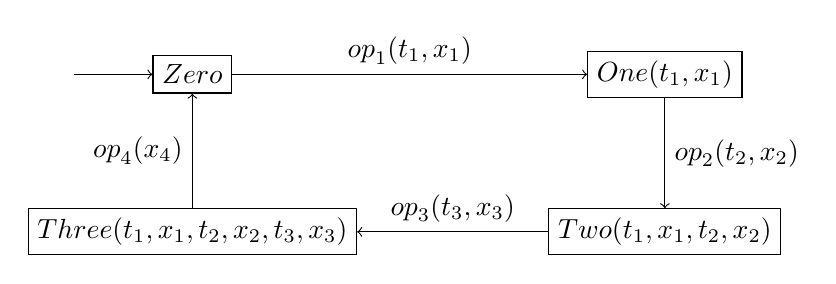
\begin{tikzpicture}[xscale = 1]
\draw (0,0) node[draw] (zero) {$\sm{Zero}$};
\draw[->] (zero) ++ (-1.5, 0) -- (zero);
%
\draw (zero)++(6,0) node[draw] (one) {$\sm{One}(\sm{t}_1, \sm{x}_1)$};
\draw[->] (zero)  -- node[above] {$\sm{op}_1(\sm{t}_1, \sm{x}_1)$} (one); 
%
\draw (one)++(0, -2) node[draw] (two) 
  {$\sm{Two}(\sm{t}_1, \sm{x}_1, \sm{t}_2, \sm{x}_2)$};
\draw[->] (one)  -- node[right] {$\sm{op}_2(\sm{t}_2, \sm{x}_2)$} (two); 
%
\draw (two)++(-6, 0) node[draw] (three) 
  {$\sm{Three}(\sm{t}_1, \sm{x}_1, \sm{t}_2, \sm{x}_2, \sm{t}_3, \sm{x}_3)$};
\draw[->] (two)  -- node[above] {$\sm{op}_3(\sm{t}_3, \sm{x}_3)$} (three); 
%
%% \draw (three)++(0,-2) node[draw] (threeX) 
%%   {$\sm{ThreeX}(\sm{y}_1, \sm{y}_2, \sm{y}_3)$};
\draw[->] (three)  -- node[left] {$\sm{op}_4(\sm{x}_4)$} (zero); 
%
%% \draw (threeX)++(-4,0) node[draw] (twoX) {$\sm{TwoX}(\sm{y}_1, \sm{y}_2)$};
%% \draw[->] (threeX)  -- node[above] {$\overline{\sm{op}}_3()$} (twoX); 
%% %
%% \draw (twoX)++(-3.5,0) node[draw] (oneX) {$\sm{OneX}(\sm{y}_1)$};
%% \draw[->] (twoX)  -- node[above] {$\overline{\sm{op}}_2()$} (oneX);
%% \draw [->] (oneX)  -- node[below] {$\overline{\sm{op}}_1()$} (zero);
\end{tikzpicture}
\end{center}
%
The final |op| operation, |op|\s4 in the above figure, applies the |sync|
method of the synchronisation specification object to the parameters $\sm x_1,
\ldots, \sm x_k$ to obtain the results $\sm y_1, \ldots, \sm y_k$; it stores
the first $k-1$ in appropriate |returns|\s{i} arrays, and returns $\sm y_k$
itself.  In the case $k=4$, it has definition:
%
\begin{scala}
  def op£\s4£(x£\s4£: A£\s4£): B£\s4£ = {
    require(state.isInstanceOf[Three]); val Three(t£\s1£, x£\s1£, t£\s2£, x£\s2£, t£\s3£, x£\s3£) = state
    val (y£\s1£, y£\s2£, y£\s3£, y£\s4£) = SyncSpec.sync(x£\s1£, x£\s2£, x£\s3£, x£\s4£) 
    returns£\s1£(t£\s1£) = Some(y£\s1£); returns£\s2£(t£\s2£) = Some(y£\s2£); returns£\s3£(t£\s3£) = Some(y£\s3£)
    state = Zero; y£\s4£
  }
\end{scala}
%
Each $\overline{\sm{op}}_i$ operation retrieves the result from the
corresponding |returns|\s{i} array.
